\documentclass[12pt]{article}

\pagestyle{empty}
\setcounter{secnumdepth}{2}
%----------------------------------------------------------------------------------------
%   Packages and configurations
%----------------------------------------------------------------------------------------
\usepackage[dutch]{babel}
\usepackage{hyperref} %Allow for references
\hypersetup{
    colorlinks,
    citecolor=black,
    filecolor=black,
    linkcolor=black,
    urlcolor=black
} %Set up hyperlink colours.
\newcommand{\sectionbreak}{\clearpage} % Should start every section on its own page
\usepackage{geometry} % Required to change the page size to A4
\geometry{a4paper} % Set the page size to be A4 as opposed to the default US Letter
\usepackage{chngpage}
\usepackage{appendix}
%REMOVE IF HEADER/FOOTER BROKEN
\usepackage{fancyhdr} % Required for custom headers
\usepackage{extramarks} % Required for headers and footers
\usepackage{lastpage} % Required to determine the last page for the footer
%-----------------1
\topmargin=0cm
\oddsidemargin=0cm
\textheight=22.0cm
\textwidth=16cm
\parindent=0cm
\parskip=0.15cm
\topskip=0truecm
\raggedbottom
\abovedisplayskip=3mm
\belowdisplayskip=3mm
\abovedisplayshortskip=0mm
\belowdisplayshortskip=2mm
\normalbaselineskip=12pt
\normalbaselines
\usepackage{listings}
\usepackage[svgnames,table,xcdraw]{xcolor}
\lstset { 
    language=C,
    frame=single,
    escapeinside={\%*}{*)}, 
    breaklines=true,  
    backgroundcolor=\color{black!5},
    basicstyle=\footnotesize,
    commentstyle=\color{mygreen},
    numberstyle=\tiny\color{mygray},
    rulecolor=\color{black},
    keywordstyle=\color{blue},
}
\definecolor{mygreen}{rgb}{0,0.6,0}
\definecolor{mygray}{rgb}{0.5,0.5,0.5}
\definecolor{mymauve}{rgb}{0.58,0,0.82}
\usepackage{wasysym}
\pagestyle{fancy}
\lhead{\textsc{Beckett}, \textsc{van Abkoude}, \textsc{West} \& \textsc{Mathijssen}} % Top left header
\rhead{Opdrachten week 1} % Top center header
\lfoot{
\includegraphics[height=0.8cm]{avans}} % Bottom left footer
\cfoot{} % Bottom center footer
\rfoot{Pagina\ \thepage} % Bottom right footer
\renewcommand\headrulewidth{0.4pt} % Size of the header rule
\renewcommand\footrulewidth{0.4pt} % Size of the footer rule
\usepackage{graphicx} % Required for including pictures

\usepackage{float} % Allows putting an [H] in \begin{figure} to specify the exact location of the figure
\usepackage{wrapfig} % Allows in-line images such as the example fish picture
\usepackage{lipsum} % Used for inserting dummy 'Lorem ipsum' text into the template
\usepackage{pdfpages}
\usepackage[font={footnotesize}]{caption}
\graphicspath{ {../Images/Logos/}{../Images/}{../Images/Week1/} }
\setlength\parindent{0pt} % Removes all indentation from paragraphs
%\usepackage{showframe}
\newcommand*{\SignatureAndDate}[1]{%
    \par\noindent\makebox[2.5in]{\hrulefill} \hfill\makebox[2.0in]{\hrulefill}%
    \par\noindent\makebox[2.5in][l]{#1}      \hfill\makebox[2.0in][l]{Date}%
}%Signature package
\begin{document}
\begin{titlepage}
\pagenumbering{Roman}
\newcommand{\HRule}{\rule{\linewidth}{0.5mm}} % Defines a new command for the horizontal lines, change thickness here

\center % Center everything on the page


\includegraphics[height=3cm] {avans}\\% Include a department/university logo - this will require the graphicx package
\textsc{\Large Avans Hogeschool Breda}\\[0.5cm] % Major heading such as course name
\textsc{\large Intelligente wireless sensornetwerken }\\[0.5cm] % Minor heading such as course title
\HRule \\[0.4cm]
{ \huge \bfseries Opdrachten week 1}\\[0.4cm] % Title of your document
\HRule \\[1.5cm]

\begin{minipage}{0.4\textwidth}
\begin{flushleft} \large
\emph{Auteurs:}\\
Guus \textsc{Beckett} \\% Your name 
Jim \textsc{van Abkoude} \\
Julian \textsc{West} \\
Joris \textsc{Mathijssen}
\end{flushleft}
\end{minipage}
~
\begin{minipage}{0.4\textwidth}
\begin{flushright} \large
\emph{Docenten:} \\
Diederich \textsc{Kroeske} \\ % Supervisor's Name
Andries \textsc{van Dongen} \\ % Supervisor's Name
\end{flushright}
\end{minipage}\\[4cm]

{\large \today}\\[3cm] % Date, change the \today to a set date if you want to be precise

Versie: 0.2.0

\vfill % Fill the rest of the page with whitespace

\end{titlepage}

\clearpage
% \section*{Voorwoord}
% \addcontentsline{toc}{section}{Voorwoord}

% Guus Beckett \& Jim van Abkoude \\
% \today \\
% Breda
% \newpage
% \section*{Samenvatting}
% \addcontentsline{toc}{section}{Samenvatting}
% \lipsum[0-2]
% \newpage
% \tableofcontents
% \newpage
\pagenumbering{arabic}
\section*{Opdracht 1}
\begin{quote}
Bij het loggen van data is een correcte time-stamp van belang. In bijlage 1 is een voorbeeld sketch gegeven waarbij de Arduino een nauwkeurige time-stamp van een NTP server ophaalt. Klopt de code met het NTP protocol? Bewerk de code zodat deze connect naar een tijdserver in NL (nl.pool.ntp.org), inclusief DNS query.
\end{quote}
\lstinputlisting{../CodeWeek1/NTP/NTPupdate.cpp}
\newpage
\section*{Opdracht 5}
\begin{quote}
Onderzoek met Postman en de HUE Api hoe je met het Philips HUE systeem moet communiceren. Gebruik de CLIP API Debugger (zie HUE API ‘Getting Started’) om met een lamp te communiceren. Kun je de lamp aan/uit zetten? Of dimmen?
\end{quote}
We hebben met CLIP API Debugger gebruikt om PUT en GET request te sturen naar de lamp.\\
We begonnen met een /api/1234 GET request. (Zie figuur 1) We kregen hier als antwoord terug dat de gebruiker geen toegang had. (Zie figuur 2)
\begin{figure}[h!]
  \centering
      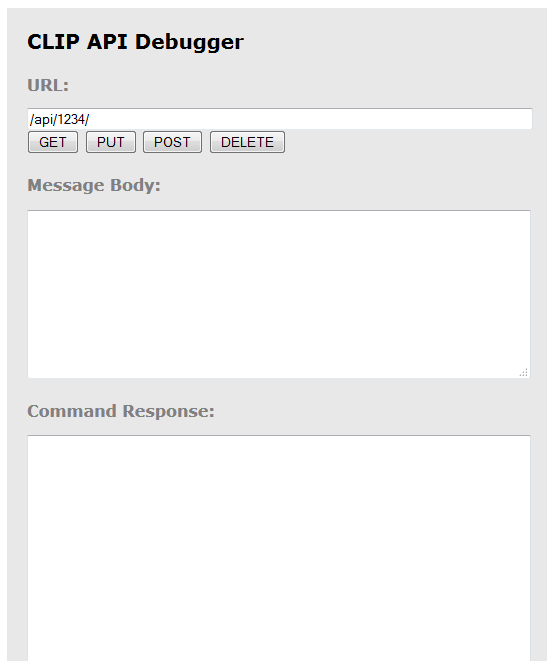
\includegraphics[width=0.3\textwidth]{stap1}
  \caption{GET request naar 192.168.1.2/api/1234}
\end{figure}
\\
\begin{figure}[h!]
  \centering
      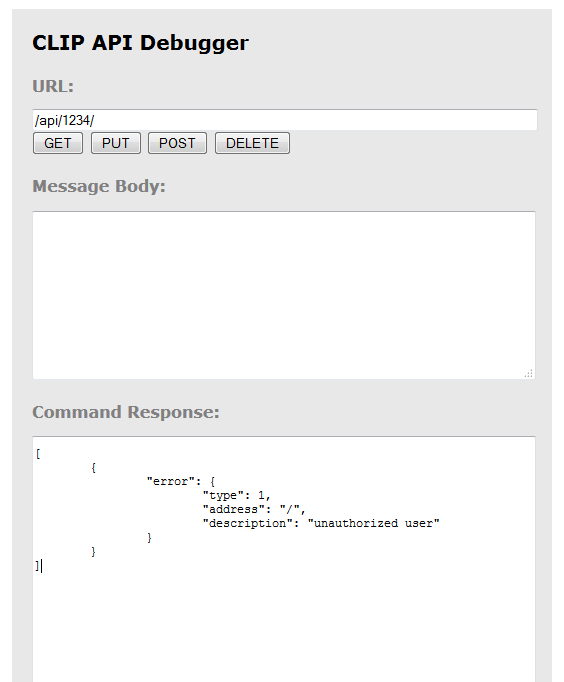
\includegraphics[width=0.3\textwidth]{stap2}
  \caption{Antwoord voor request 192.168.1.2/api/1234, unauthorized user}
\end{figure}
\newpage
Hierna stuurde we een GET request naar 192.168.1.2/api/. Hier kregen we een succesvol antwoord terug. We kregen in het antwoord te zien dat de ussername 'newdeveloper' is.
\begin{figure}[h!]
  \centering
      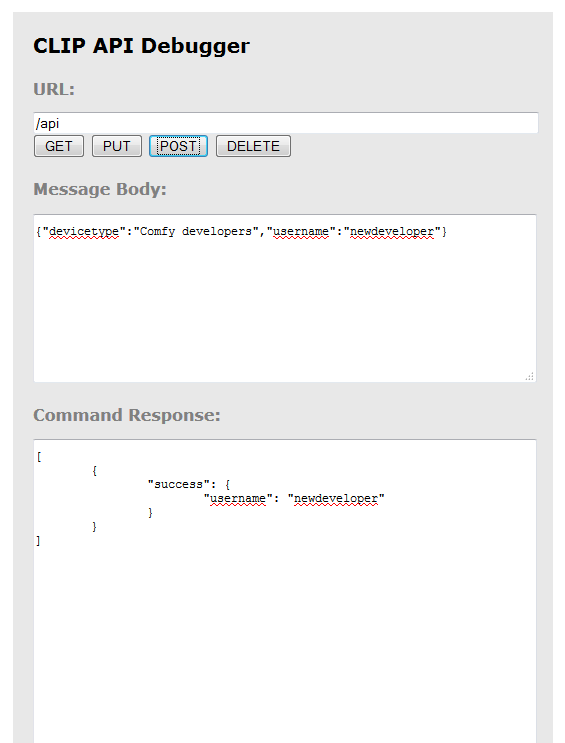
\includegraphics[width=0.35\textwidth]{stap3}
  \caption{GET Request naar 192.168.1.2/api/, Success; ussername: newdeveloper }
\end{figure}
\\
Hierna gebruikte we newdeveloper om de lichten aan te sturen. Hier kregen we een succes terug met allemaal data dit hier onder te lezen valt.
\begin{figure}[h!]
  \centering
      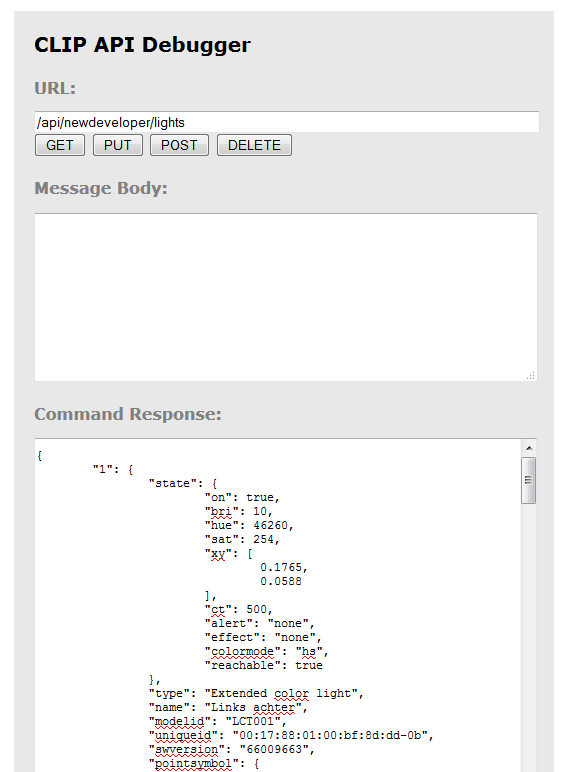
\includegraphics[width=0.35\textwidth]{stap4}
  \caption{Request naar 192.168.1.2/api/newdeveloper/lights}
\end{figure}
\newpage
Zodra we de verbonden zijn met de bridge en een GET request sturen naar \\\textit{192.168.1.2/api/newdeveloper/lights} krijgen we de volgende output
\begin{lstlisting}
{
    "1": {
        "state": {
            "on": true,
            "bri": 10,
            "hue": 46260,
            "sat": 254,
            "xy": [
                0.1765,
                0.0588
            ],
            "ct": 500,
            "alert": "none",
            "effect": "none",
            "colormode": "hs",
            "reachable": true
        },
        "type": "Extended color light",
        "name": "Links achter",
        "modelid": "LCT001",
        "uniqueid": "00:17:88:01:00:bf:8d:dd-0b",
        "swversion": "66009663",
        "pointsymbol": {
            "1": "none",
            "2": "none",
            "3": "none",
            "4": "none",
            "5": "none",
            "6": "none",
            "7": "none",
            "8": "none"
        }
    },
    "2": {
        "state": {
            "on": true,
            "bri": 143,
            "hue": 4626,
            "sat": 254,
            "xy": [
                0.6269,
                0.3574
            ],
            "ct": 500,
            "alert": "none",
            "effect": "none",
            "colormode": "hs",
            "reachable": true
        },
        "type": "Extended color light",
        "name": "Rechts achter",
        "modelid": "LCT001",
        "uniqueid": "00:17:88:01:00:bf:7f:36-0b",
        "swversion": "66009663",
        "pointsymbol": {
            "1": "none",
            "2": "none",
            "3": "none",
            "4": "none",
            "5": "none",
            "6": "none",
            "7": "none",
            "8": "none"
        }
    },
    "3": {
        "state": {
            "on": true,
            "bri": 10,
            "hue": 46260,
            "sat": 254,
            "xy": [
                0.1765,
                0.0588
            ],
            "ct": 500,
            "alert": "none",
            "effect": "none",
            "colormode": "hs",
            "reachable": true
        },
        "type": "Extended color light",
        "name": "Links voor",
        "modelid": "LCT001",
        "uniqueid": "00:17:88:01:00:bf:90:49-0b",
        "swversion": "66009663",
        "pointsymbol": {
            "1": "none",
            "2": "none",
            "3": "none",
            "4": "none",
            "5": "none",
            "6": "none",
            "7": "none",
            "8": "none"
        }
    },
    "4": {
        "state": {
            "on": true,
            "bri": 254,
            "hue": 60050,
            "sat": 254,
            "xy": [
                0.5928,
                0.25
            ],
            "alert": "none",
            "effect": "none",
            "colormode": "hs",
            "reachable": true
        },
        "type": "Color light",
        "name": "Bloom rechts voor",
        "modelid": "LLC012",
        "uniqueid": "00:17:88:01:00:c3:61:90-0b",
        "swversion": "66009461",
        "pointsymbol": {
            "1": "none",
            "2": "none",
            "3": "none",
            "4": "none",
            "5": "none",
            "6": "none",
            "7": "none",
            "8": "none"
        }
    },
    "5": {
        "state": {
            "on": true,
            "bri": 50,
            "hue": 4626,
            "sat": 254,
            "xy": [
                0.703,
                0.296
            ],
            "alert": "none",
            "effect": "none",
            "colormode": "hs",
            "reachable": false
        },
        "type": "Color light",
        "name": "Bloom links achter",
        "modelid": "LLC012",
        "uniqueid": "00:17:88:01:00:c3:61:ba-0b",
        "swversion": "66009461",
        "pointsymbol": {
            "1": "none",
            "2": "none",
            "3": "none",
            "4": "none",
            "5": "none",
            "6": "none",
            "7": "none",
            "8": "none"
        }
    }
}
\end{lstlisting}
\newpage
\section*{Opdracht 6}
\begin{quote}
Implementeer een sketch die de lamp uit de vorige opdracht kan schakelen/dimmen door het drukken
op (hardware) schakelaars die op de Arduino zijn aangesloten.
\end{quote}
Zodra we de verbonden zijn met de bridge sturen we een PUT request naar \\\textit{192.168.1.2/api/newdeveloper/lights/4/state} Hier bij geven we de channel en state mee. State word bepaald door de kopjes op de Arduino uit te lezen. 
\begin{figure}[h!]
  \centering
      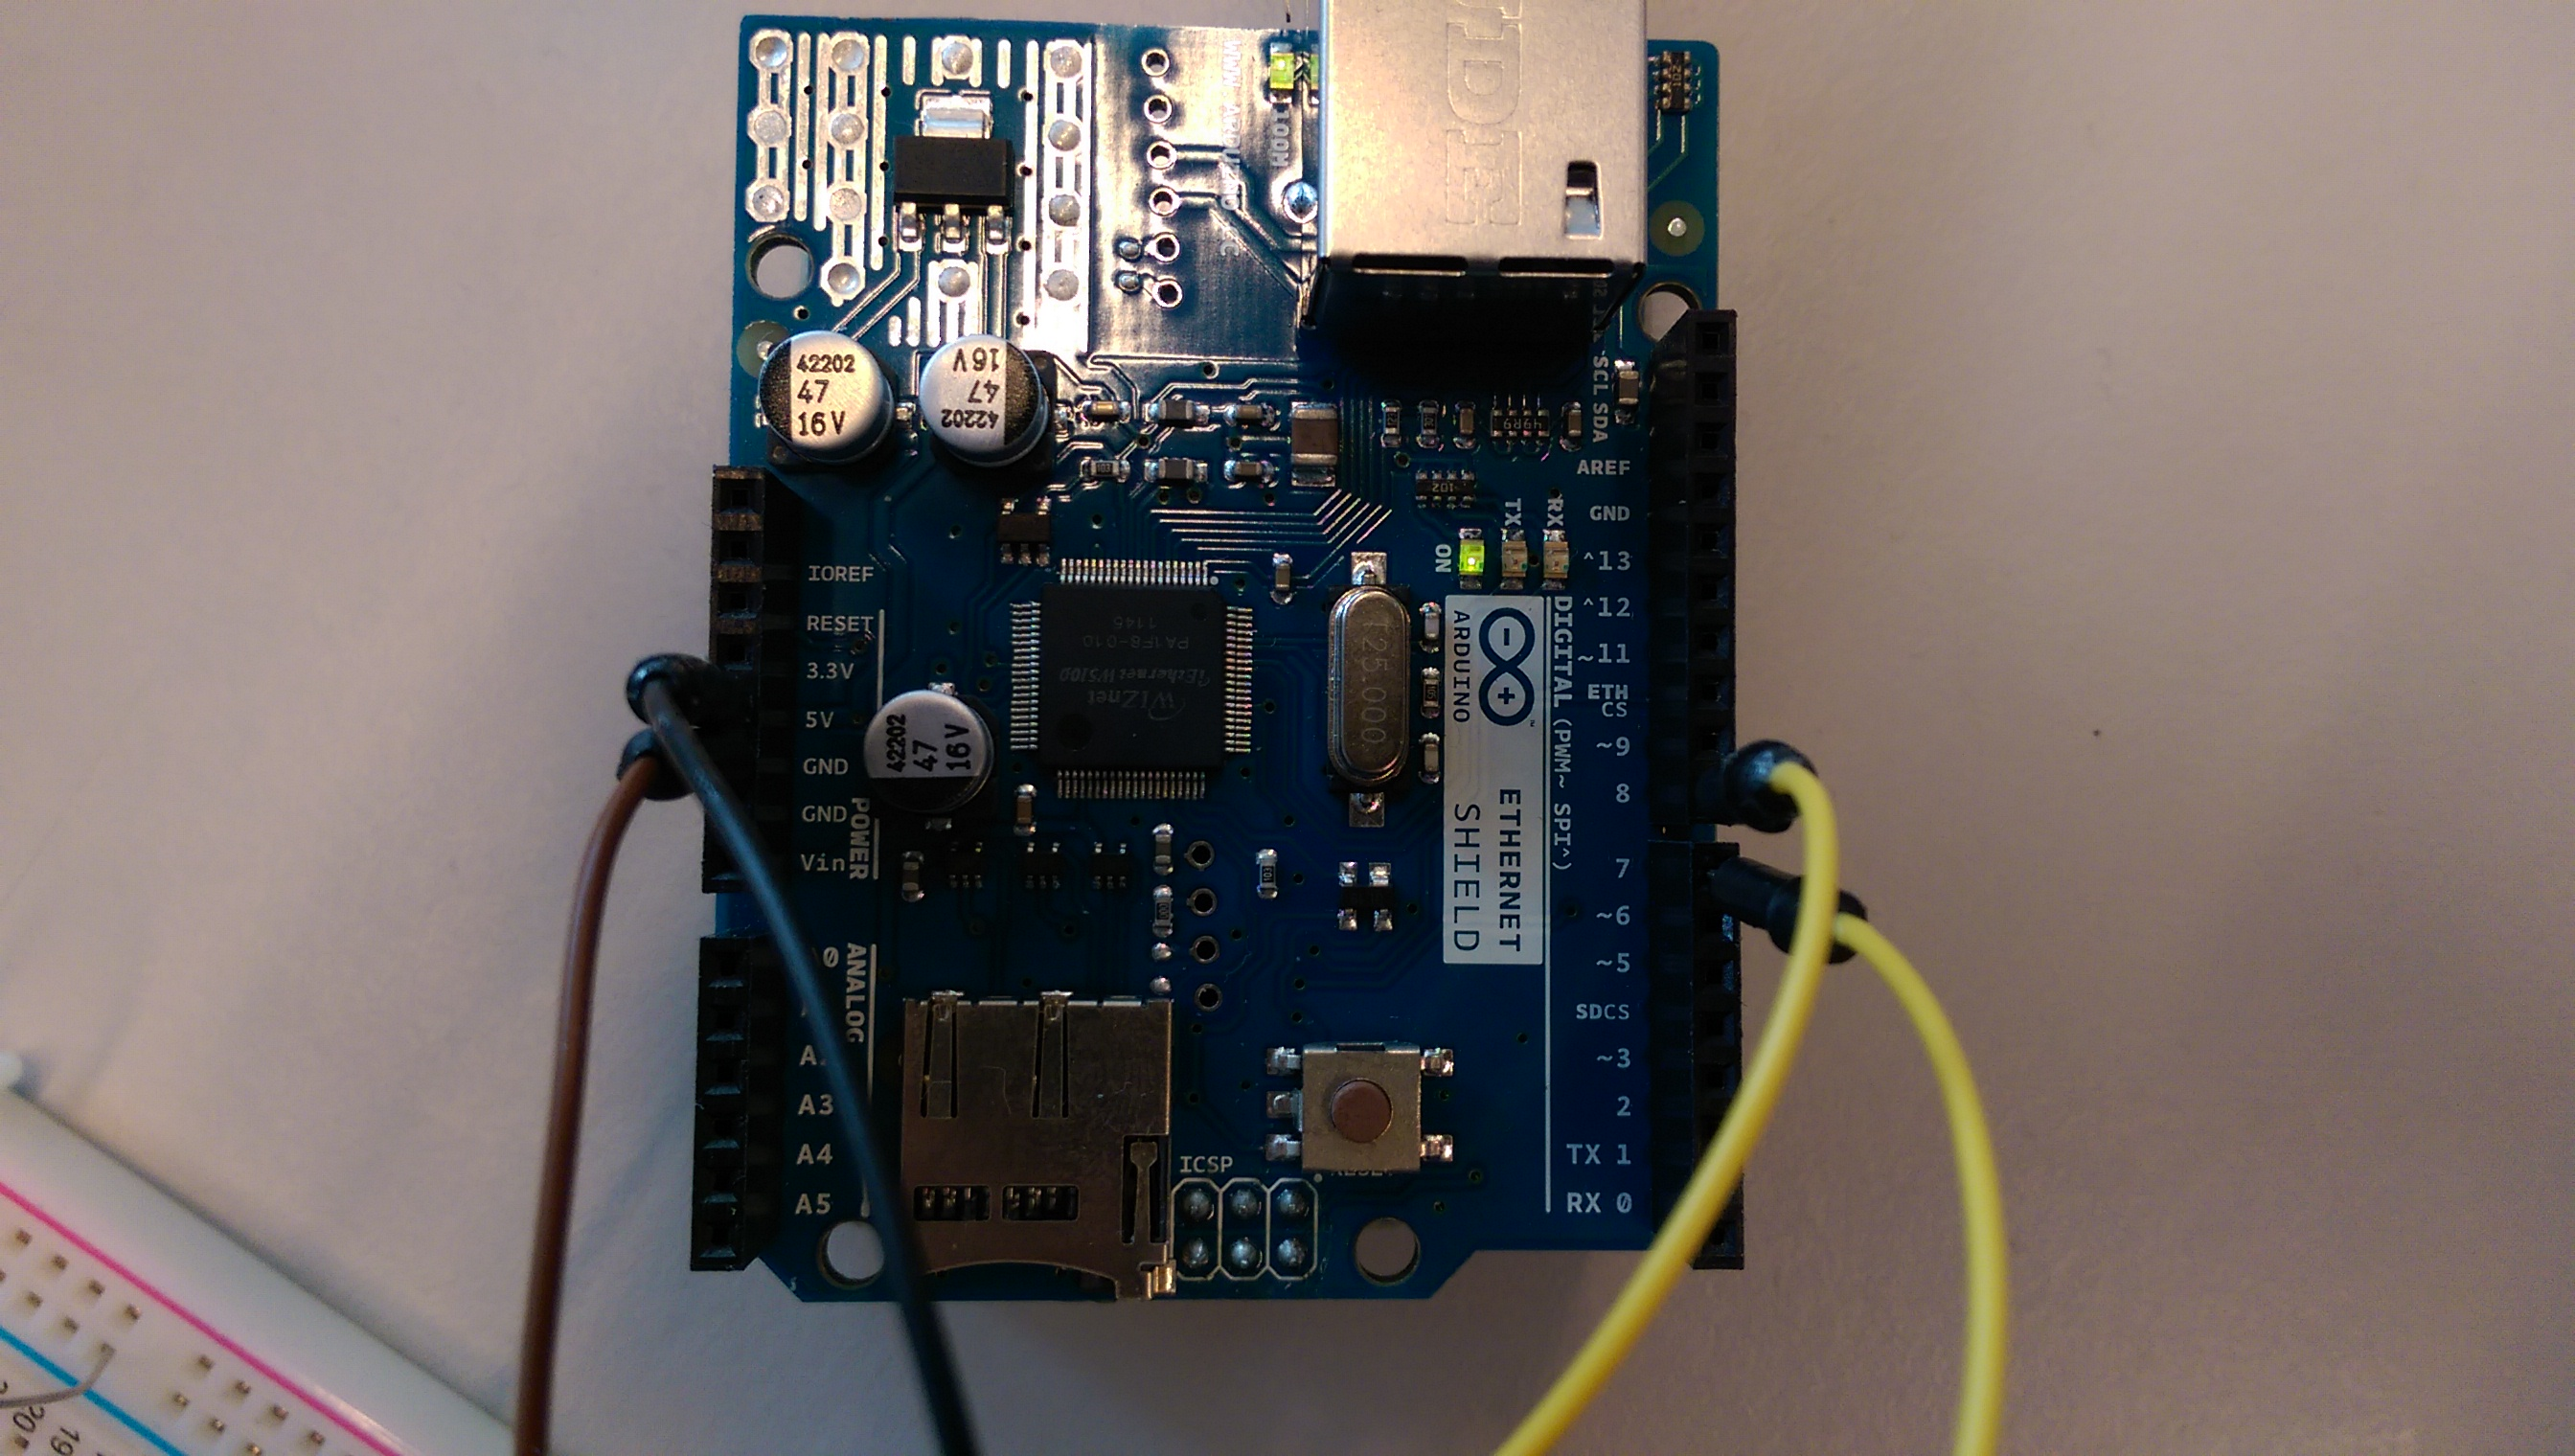
\includegraphics[width=0.7\textwidth]{IMAG0046}
  \caption{Pin 7 \& 8 zijn de pins die de input van de knopjes ontvangen op de Arduino.}
\end{figure}
\begin{figure}[h!]
  \centering
      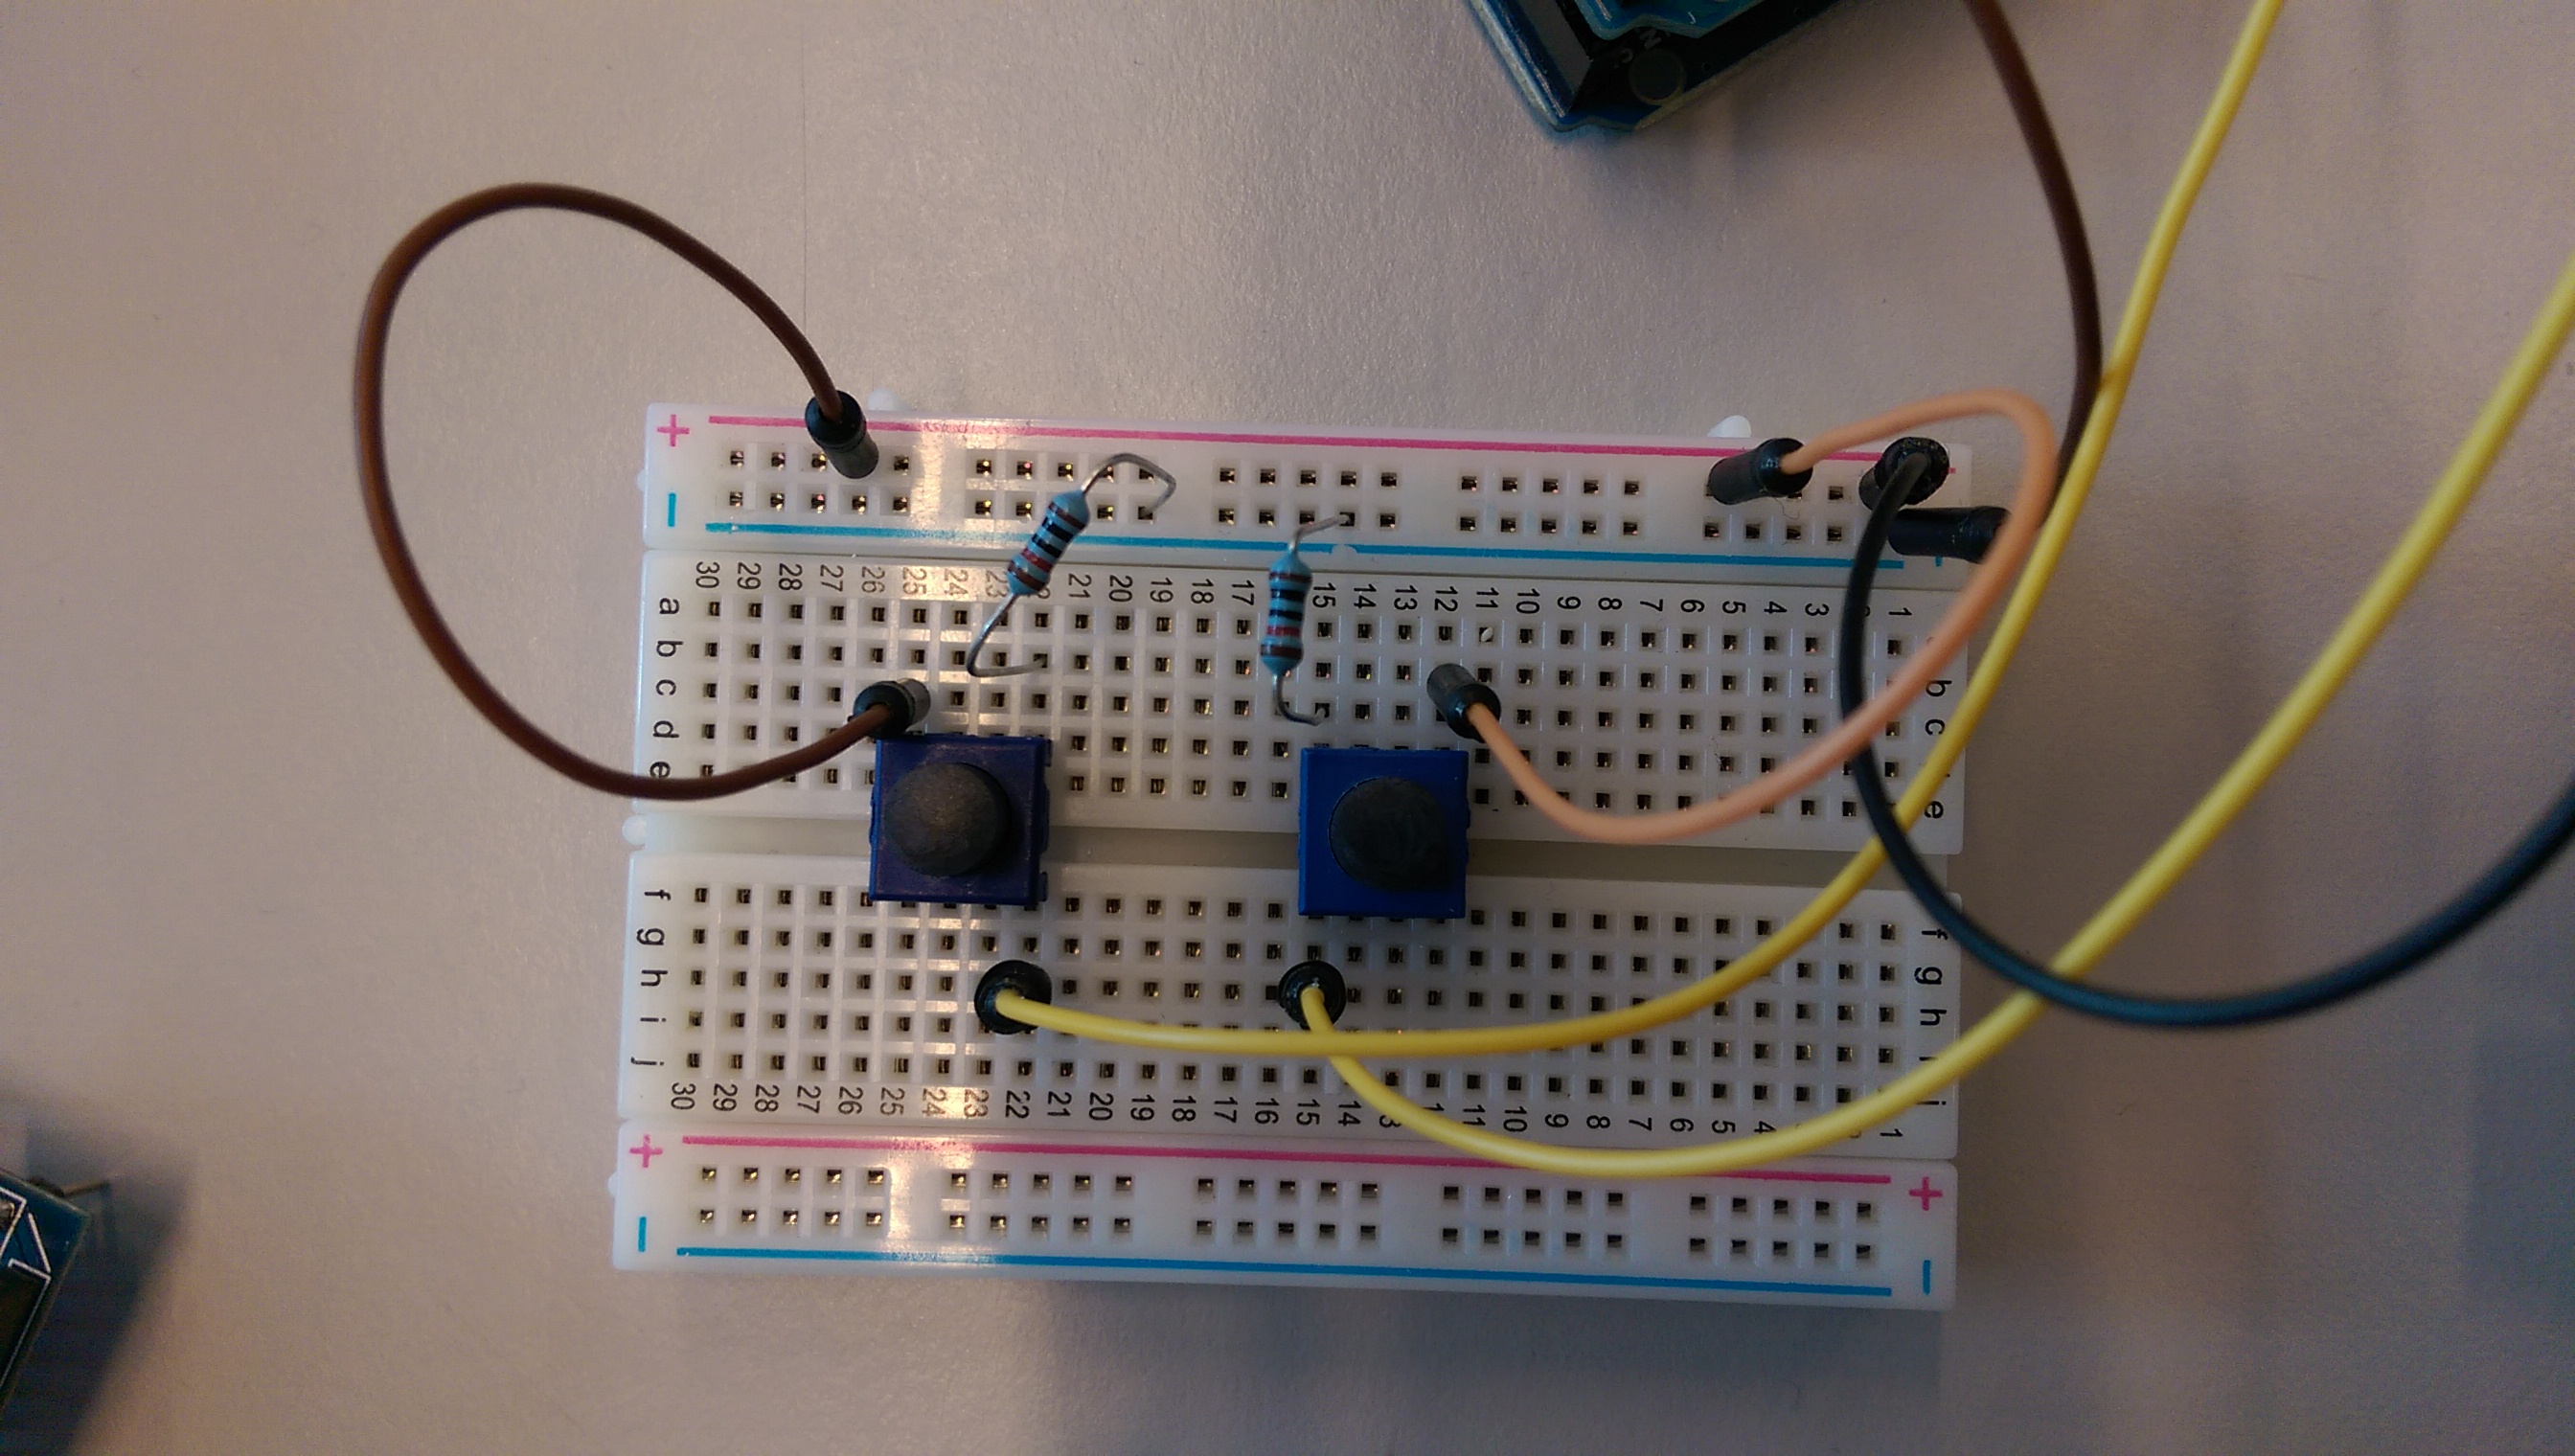
\includegraphics[width=0.7\textwidth]{IMAG0048}
  \caption{Breadbord met de knopjes. Waar de knopjes op geprikt zijn.}
\end{figure}
\newpage
\lstinputlisting{../CodeWeek1/HUE/KnoppenUitlezen.cpp}
\end{document}
